\def\year{2015}
%File: formatting-instruction.tex
\documentclass[letterpaper]{article}
\usepackage{aaai}
\usepackage{times}
\usepackage{helvet}
\usepackage{courier}

\usepackage[colorlinks=true,linkcolor=blue]{hyperref}	% For hyper links
\usepackage{caption}
\usepackage{subcaption}
\usepackage{bbm}

\usepackage{CJKutf8} 
\usepackage{ucs} 
\usepackage[encapsulated]{CJK} 
\newcommand{\myfont}{gbsn}
\usepackage[usenames]{color}
\newcommand{\red}[1]{\textcolor{red}{#1}}

\usepackage{amssymb,amsmath}
\usepackage{graphicx}

\frenchspacing
\setlength{\pdfpagewidth}{8.5in}
\setlength{\pdfpageheight}{11in}
\pdfinfo{
/Title Burst Learning to Discover Interesting Moments in Social Media Streams
/Author Author 1, Author 2, Author 3}
%/Author Cody Buntain, Jimmy Lin, Jen Golbeck}
\setcounter{secnumdepth}{0}  
 \begin{document}
% The file aaai.sty is the style file for AAAI Press 
% proceedings, working notes, and technical reports.
%
\title{Burst Learning to Discover Interesting Moments in Social Media Streams}
%\author{Cody Buntain, Jimmy Lin \and Jen Golbeck \\
%Department of Computer Science \\
%University of Maryland \\
%College Park, Maryland 20742 USA \\
%}
\author{Author 1\\
Dept. \\
University \\
Address \\
%\AND
%Author 2 and Author 3
%Dept. \\
%University \\
%Address
}
\maketitle
\begin{abstract}
\begin{quote}
This paper introduces a general technique for identifying interesting and compelling moments in social media streams without the need for any domain-specific information or seed keyword lists.
We leverage machine learning to model temporal patterns around bursts in Twitter's public sample stream and build a classifier to identify tokens experiencing these bursts.
Since many events are also interesting moments, we are also able to subsume some event detection tasks and achieve a measure of language agnosticism and general flexibility current techniques lack. 
To demonstrate our approach's potential, we compare a baseline event-detection system with our language-agnostic algorithm in detecting a number of key moments across three major sporting competitions:\ the 2013 World Series, 2014 Super Bowl, and 2014 World Cup.
Results from this comparison show our method demonstrates similar performance in this sports domain without the need for pre-specified tokens.
We then go further by applying our sports-based models to the task of identifying earthquakes in Japan and show our method detects large spikes in earthquake-related tokens within two minutes of the actual event.
\end{quote}
\end{abstract}

% A category with the (minimum) three required fields
%\category{H.2.8}{Database Applications}{Data Mining}
%\category{\\H.3.3}{Information Search and Retrieval}{Information Filtering}
%
%\keywords{event detection, twitter, social networks, temporal features}

\section{Introduction}

Though researchers have presented a multitude of methods for adapting social media streams to informational and news sources for journalists or first responders, many current social media-based event detection systems rely on manually defined keywords to detect interesting events.
Though straightforward and capable, such approaches are constrained only to those types of events for which they have defined keywords or other specific information, potentially missing impactful but unanticipated events.
Part of the difficulty in a journalist's job is to identify these unexpected but newsworthy occurrences.
For instance, one can follow the frequency of words like ``goal'' on Twitter during the 2014 World Cup to detect when goals are scored \cite{Cipriani2014}, but interesting occurrences like penalties or missed goals would be missed.
One might respond to this weakness by tracking additional penalty-related tokens, but this approach would still be unable to identify \emph{unexpected} moments like Luis Suarez's biting Giorgio Chiellini during the Uruguay-Italy World Cup match; who would have thought to include ``bite'' as a relevant token during that event?
Furthermore, relying on predefined keywords restricts these systems to those languages represented in the seed keyword set, a significant issue for international events like the World Cup.
Given the shear volume of social media data (hundreds of thousands of comments, statuses, and photos generated per minute on Facebook alone as of 2012 \cite{Pring2012}), one could instead forgo seed keywords completely and track bursts in overall message volume (as with Vasudevan et al. \cite{vasudevan2013twitter}) and sacrifice semantic information about detected events (as one would need to extract keywords causing such bursts manually).
In this paper, we propose leveraging machine learning to reap the benefits of both techniques.

To explore this integration, we introduce LABurst (short for language-agnostic burst detection), a general learning method to model the temporal signatures of keyword bursts in social media streams.
We then use LAburst to track the number of keywords experiencing bursts in a particular moment, which serves as a predictor of an interesting or high-impact occurrence. 
In contrast to existing work, our approach processes \emph{unfiltered} social media streams, discovers high-impact moments in those streams without prior knowledge of the target events, \emph{and} yields keywords describing these discovered events.
Illustrating this flexibility is a collection of experiments on Twitter streams surrounding key moments in large sporting competitions and natural disasters.
These experiments include comparisons between LABurst and two existing burst detection methods: a volume-centric burst detection technique, and a similar technique with a pre-determined set of sports-related keywords.

This work makes the following contributions:
%
\begin{itemize}
\item We propose a feature set and classifier for the language-agnostic discovery of impactful or interesting moments in the Twitter public sample stream. Importantly, our approach does {\it not} require a list of manually-defined keywords as input,

\item We demonstrate our approach's performance is both competitive with existing techniques and more flexible, and

\item We can transfer our models across disparate domains and still maintain comparable levels of performance to domain-specific systems.
\end{itemize}

\section{Related Work}
\label{sect:relatedWork}

Though we are focusing on the slightly different problem of identifying ``interesting moments'' in social media streams, we still build on much of the same work as classical event detection, which has fascinated researchers for over twenty years.
This subfield has evolved to integrate the latest available techniques and data sources, starting from early digital newsprint to blogs and now social media.
Early stages of this research began in the mid-nineties with the Topic Detection and Tracking (TDT) initiative.
These programs demonstrated feasibility in detecting new topics from traditional media sources, but as Allan, Papka, and Lavrenko discussed in 1998, these approaches required additional work to see real success \cite{allan1998line}.
Even in that early work, Allan et al. were already discussing the tradeoffs of using pre-defined keyword sets and event classes when detecting new events.
%It is also important to note that, at this nascent stage, topic detection and event detection were relatively synonymous.

Though this early research focused primarily on topic detection from newsprint and traditional media sources, Kleinberg's 2002 paper altered the landscape by applying topic detection to non-traditional data sources like his personal email archive and by introducing what appears to be the first real treatment of burst analysis in ``document streams that arrive continuously over time'' rather than  static collections \cite{Kleinberg:2002:BHS:775047.775061}. 
Despite introducing the streaming context, Kleinberg cast topic detection as a retrospective, state-based optimization problem.
He then leveraged existing work on hidden Markov models (HMMs) to find sequences of high usage keywords, or bursts, from which he could detect events (and construct complex nested states to develop event hierarchies).
Kleinberg's examination here laid much of the foundation for the focus on topic bursts that characterized much of the proceeding research in this area.

Following from Kleinberg's work and the increasing size of digital content on the Internet, several new approaches to topic detection emerged.
Notably, topic detection divided into two distinct tasks: identifying topics in data via algorithms like Latent Dirichlet Allocation (LDA) \cite{blei2003latent} and detecting events from text.
Our research focuses on events rather than topics, so early event detection work like that from Fung et al. in 2005 is especially interesting \cite{Fung:2005:PFB:1083592.1083616}.
Fung et al. extended Kleinberg's burst detection scheme by identifying bursty keywords from digital newspapers and clustering these keywords into groups to identify bursty events, which displayed success in identifying trending events in an English-language newspaper from Hong Kong.

%Along with new interest in burst-centric research, another important trend starting around this time was the integration of additional data sources beyond traditional newsprint, specifically blog content.
%Blogs offered direct insight into the social consciousness in a way that was previously unavailable via traditional media since blogs include a great deal of social information regarding the author.
%Zhao et al. took advantage of this additional social information in their 2007 work on flow-based event detection from 2007 \cite{Zhao2007}.
%By integrating this social data with the textual and temporal techniques described above, Zhao et al. were able to identify events with high accuracy in two social datasets: the Enron email dataset and the Dailykos dataset.
%Similarly, Bansal's group from the University of Toronto developed the Blogscope project to identify trending and bursty keywords by location as well as time across the entire ``blogosphere'' \cite{Bansal:2007:BSO:1325851.1326028,Bansal:2007:BSA:1242572.1242802}.

%\subsection{Event Detection in Microblogs}

Soon after, the research community began experimenting with alternative media sources like blogs, but real gains came when microblogging platforms began their rise in popularity.
These microblogging platforms include Twitter and Sina Weibo and are characterized by constrained post sizes (e.g., Twitter constrains user posts to 140 characters) and broadcasting publicly consumable information.
Since their rise, a great deal of research has explored how data posted to these networks can be leveraged for social good projects like event detection.
Much of this work, however, is retrospective in nature and focuses on detecting events after the fact rather than utilizing one of the real advantages in these social networks: unlike newspapers and blogs, these networks produce huge volumes of information that can be processed in \emph{real time}.

One of the most well-known works in detecting events from microblog streams is Sakaki, Okazaki, and Matsuo's 2010 paper on detecting earthquakes in Japan using Twitter \cite{Sakaki:2010:EST:1772690.1772777}.
Sakaki et al. show that not only can one detect earthquakes on Twitter but also that it can be done simply by tracking frequencies of earthquake-related tokens.
Surprisingly, this approach can outperform geological earthquake detection tools since digital data propagates faster than tremor waves in the Earth's crust.
Though this research is limited in that it requires pre-specified tokens and is highly domain- and location-specific (Japan has a high density of Twitter users, so earthquake detection may perform less well in areas with fewer Twitter users), it demonstrates a significant use case and the potential of such applications.

Along with Sakaki et al., 2010 saw two other relevant papers: Lin et al.'s construction of a probabilistic popular event tracker \cite{Lin:2010:PSM:1835804.1835922} and Petrovi\'{c}, Osborne, and Lavrenko's application of locality-sensitive hashing (LSH) for detecting first-story tweets from Twitter streams \cite{Petrovic:2010:SFS:1857999.1858020}.
Lin's work is interesting for a number of reasons: first, it circumvents the need for language model-based stop word lists by using probabilistic models to discriminate between common and informational tokens.
Secondly, Lin's integration of social and structural features into the event detection task demonstrated that real performance enhancements can be gained through non-textual features.
Thirdly, their paper relates well to Kleinberg's initial work on bursty topic detection by illustrating how his state machine approach is a degenerate case of the PET model.
Like the majority of its contemporary systems, however, PET also requires seeding with a pre-specified list of tokens to guide its event detection and concentrates on retrospective per-day topics and events.

In contrast, Petrovi\'{c} and his colleagues' clustering research in Twitter avoids the need for seed keywords and retrospective analysis by instead focusing on the practical considerations of clustering large streams of data quickly.
That is, rather than construct a probabilistic mixture model for each token, Petrovi\'{c} focuses on methods for clustering tweets that contain similar tokens into topical clusters.
While typical clustering algorithms require distance calculations for all pairwise messages, LSH facilitates rapid clustering at the scale necessary to support event detection in Twitter streams by restricting the number of tweets compared to only those within some threshold of similarity.
Once these clusters are generated, Petrovi\'{c} was able to track their growth over time to determine impact for a given event.
This research was originally unique in that it was one of the early methods that did not require pre-specified seed tokens for detecting events and has been very influential in the field, resulting in a number of additional publications to demonstrate its utility in breaking news and for high-impact crisis events \cite{osborne2014real,petrovic2013can,6601695}.
That being said, a key weakness in Petrovi\'{c}'s work is its reliance on semantic similarity between tweets, which limits its ability to operate in mixed-language environments.

Similar to Petrovi\'{c}, Weng and Lee's 2011 paper on EDCoW, short for Event Detection with Clustering of Wavelet-based Signals, is also able to identify events from Twitter without seed keywords \cite{weng2011event}.
After stringent filtering (removing stop words, common words, and non-English tokens), EDCoW uses wavelet analysis to isolate and identify bursts in token usage as a sliding window advances along the social media stream.
Highly significant bursts are then cast as a cross-correlation matrix against which a graph partitioning algorithm is run to construct topical clusters from bursty tokens.
Besides the heavy filtering of the input data, this approach exhibits notable similarities with the language-agnostic method we describe herein with its reliance on bursts to detect event-related tokens; the methods described in Weng and Lee's paper, however, operate in a more retrospective manner, focusing on the level of daily news rather than breaking event detection on which our research focuses.
Becker, Naaman, and Gravano's 2011 paper on identifying events in Twitter also fall under this label of retrospective analysis, but their findings also demonstrate reasonable performance in identifying events in Twitter by leveraging classification tasks to separate tweets into those on ``real-world events'' versus non-event messages \cite{becker2011beyond-tr,becker2011beyond}.
Similarly, Diao et al. also employ a retrospective technique to separate tweets into global, event-related topics and personal topics \cite{diao2012finding}.

Beyond these works, several domain-specific research efforts have targeted sporting events specifically\cite{vasudevan2013twitter,Zhao2011,lanagan2011using}.
Lanagan and Smeaton's work is of particular interest because it relies almost solely on Twitter's per-second message volume \cite{lanagan2011using}.
Though naive, this frequency approach is able to detect large bursts on Twitter in high-impact events  without reliance on complex linguist analysis and performs well in streaming contexts as little information must be kept in memory.
Unfortunately, two main disadvantages exist with this technique: first, detecting a burst would provide evidence of an event, but it would be difficult to gain insight into what that event actually was without additional processing.
Secondly, as described in their paper, a pure volumetric approach is hampered by limitations on Twitter's public stream, which has an upper limit on the number of messages per minute one can capture.

Finally, the most recent work relevant to our research is the 2013 paper by Xie et al. on TopicSketch \cite{xie2013topicsketch}.
Like us, TopicSketch's authors seek to perform real-time event detection from Twitter streams ``without pre-defined topical keywords'' by maintaining acceleration features across three levels of granularity: individual token, bigram, and total stream.
As with Petrovi\'{c}'s use of LSH, Xie et al. leverage ``sketches'' and dimensionality reduction to facilitate event detection and also relies on language-specific similarities.
Furthermore, Xie et al. focus only on tweets from Singapore rather than the worldwide stream.
In contrast, our approach is differentiated primarily in its language-agnosticism and its use of the unfiltered stream from Twitter's global network.

Despite this extensive body of research, it is worth asking how event detection on Twitter streams differs from Twitter's own offerings on ``Trending Topics,'' which they make available to all their users.
When a user visit's Twitter's website, she is immediately greeted with her personal feed as well as a listing of trending topics for her city, country, worldwide, or nearly any location she chooses.
These topics offer insight into the current popular topics on Twitter, but the main differentiating factor is that these popular topics are not necessarily connected to specific events.
Rather, popular memetic content like ``\#MyLovelifeInMoveTitles'' often appear on the list of trending topics.
Additionally, Twitter monetizes these trending topics as a form of advertising \cite{Sydell2011}.  
These trending topics also can be more high-level than the interesting moments we seek to identify: for instance, during the World Cup, particular matches or the tournament in general were identified as trending topics by Twitter, but individual events like goals or penalty cards in those matches were not.
It should be clear then that Twitter's trending topics serves a different purpose than the streaming event detection described herein.

\section{Moment Discovery Defined}
\label{sect:model}

This paper demonstrates the LABurst algorithm's ability to discover and describe impactful moments from social media streams \emph{without} pre-specified knowledge of the types or domains of these target moments.
First though, we lay LABurst's foundations by defining the problem LABurst seeks to solve and presenting the model around which LABurst is built.

\subsection{Problem Definition}

Given an unfiltered (though potentially downsampled) stream $S$ of messages $m$ consisting of various tokens $w$, our objective is to determine whether each minute $t$ contains a compelling or high-impact moment and, if so, \emph{extract} a set of tokens that describe that moment.
These tasks are difficult to perform separately because, by the time one can react with a separate analysis tool to identify relevant tokens, the moment may have passed, and to our knowledge, no existing algorithm satisfies this joint problem in the streaming context.
By focusing on individual minutes of activity, we also avoid the complexities of defining ``events'' and the hierarchies among them.

More formally, if we let $E$ denote the set of all minutes $t$ in which an interesting moment occurs, then the indicator function $\mathbbm{1}_E(S_t, t)$ takes the stream $S$ up to time $t$ and returns a $1$ for all times $t$ in which such a moment occurs, and $0$ for all other values of $t$. 
We can then define the moment discovery task as constructing a function that approximates this indicator function $\mathbbm{1}_E(S_t, t)$.
We also include a function $B_E(S_t, t)$ that returns a set of words $w$ that describe the discovered moment at time $t$ if $t \in E$ and an empty set otherwise.

To account for possible lag in experiencing the event, typing out a message about the event, and the message actually posting to a social media server, we include a parameter $\tau$ to control for tolerance of delay.
This parameter relaxes the task slightly by constructing the set $E'$ where, for all $t \in E$, $t, t+1, t+2, ..., t+\tau \in E'$.
Since our evaluation is a comparison between two methods that share the same ground truth, and controlling $\tau$ affects the ground truth consistently for both methods, comparative results should be unaffected.
In this paper, we use $\tau=2$.

False positives/negatives and true positives/negatives follow in the normal way for some candidate function $\widehat{\mathbbm{1}_{E'}}(S_t, t)$: a false positive is any time $t$ such that $\widehat{\mathbbm{1}_{E'}}(S_t, t) = 1$ and ${\mathbbm{1}_{E'}}(S_t, t) = 0$; likewise, a false negative is any $t$ such that $\widehat{\mathbbm{1}_{E'}}(S_t, t) = 0$ and ${\mathbbm{1}_{E'}}(S_t, t) = 1$.
True positives/negatives then follow as expected.

\subsection{The LABurst Model}

In LABurst, we sought to combine the language-agnostic flexibility of general burst detection techniques with the informative capabilities of pre-defined seed keyword burst detectors by leveraging machine learning to model bursts in token usage.
At a high level, we ingest a social media stream, maintain a sliding window of frequencies for \emph{each} token contained within the stream, and use the number of bursty tokens in a given minute as an indicator of the impact of that moment.
Critically, these tokens can be of any language and are \emph{neither} stemmed nor normalized.
As an example, after a goal is scored in a World Cup match, one would expect to see many different forms of the word "goal" (both different languages and different variations, such as "gooooaaal!") experiencing bursts within a minute of the score; the more such tokens experience a burst, the higher impact the event.

At a lower level, LABurst runs a sliding window over the incoming data stream $S$ and divides it into slices of a fixed number of seconds $\delta$ such that time $t_{i} - t_{i-1} = \delta$.
LABurst then combines a set number $\omega$ of these slices into a single window (with an overlap of $\omega - 1$ slices), splits each message in that window into a set of tokens, and tabulates each token's frequency.
By maintaining a list of frequency tables from the past $k$ windows up to time $t$ (see Figure \ref{fig:windowSlices}), we can construct features describing how a token's frequency changes over time and apply tools from machine learning to separate these tokens into two classes: bursty tokens $\mathbf{B}_t$, and non-bursty tokens $\mathbf{B}'_t$.
Following this classification, if the number of bursty tokens exceeds some threshold $|\mathbf{B}_t| \ge \rho$, LABurst flags this window at time $t$ as containing a high-impact moment.
In this manner, LABurst approximates the target indicator function with $\widehat{\mathbbm{1}_{E'}}(S_t, t) = |\mathbf{B}_t| \ge \rho$ and yields $\mathbf{B}_t$ as the set of descriptive tokens for the given moment.

\begin{figure}[hbtp]
\begin{center}
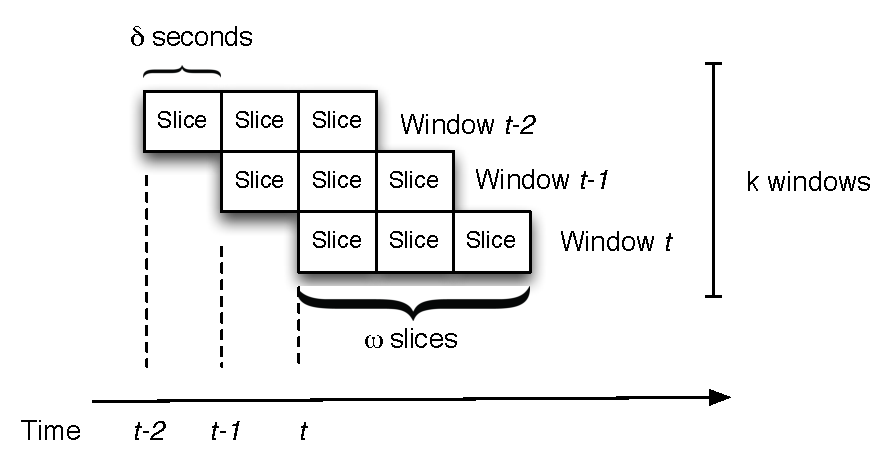
\includegraphics[width=3in]{./figures/laburst.pdf}
\caption{LABurst Sliding Window Model}
\label{fig:windowSlices}
\end{center}
\end{figure}

To avoid spurious bursts generated by endogenous network affects, it is worth noting we discard duplicate messages such as retweets or shares since existing literature shows retweets propagate extremely rapidly, potentially leading to false positives \cite{kwak2010twitter}.

\subsubsection{Temporal Features}

To capture the dynamics of how a token's usage changes, LABurst extracts a number of temporal features for each token across $k$ windows.
Each feature is normalized into the range $[0, 1]$ to avoid biases from scale.

\begin{itemize}
\item \textbf{Frequency Regression} Given the logarithm of a token's frequency at each window, take the slope of the best-fitting line.
\item \textbf{Message Frequency Regression} Given the logarithm of the number of messages in which a token appears for each window, take the slope of the best-fitting line.
\item \textbf{User Frequency Regression} Given the logarithm of the number of authors using a token for each window, take the slope of the best-fitting line.
\item \textbf{Average Frequency Difference} The difference between the token's frequency in the most recent window and the average frequency across the previous $k -1$ windows.
\item \textbf{Message Average Frequency Difference} The difference between the number of messages in which a token appears in the most recent window and the average frequency across the previous $k -1$ windows.
\item \textbf{User Average Frequency Difference} The difference between the number of users who use a token in the most recent window and the average frequency across the previous $k -1$ windows.
\item \textbf{Inter-Arrival Time} The average number of seconds between token occurrences in the previous $k$ windows.
\item \textbf{Entropy} The entropy of the set of messages containing a given token.
\item \textbf{TF-IDF} The term frequency, inverse document frequency for a each token.
\item \textbf{TF-PDF} A modified version of TF-IDF called term frequency, proportional document frequency \cite{Bun:2002:TEN:645962.674082}.
\item \textbf{BursT} Weight using a combination of a given token's actual frequency and expected token frequency \cite{Lee:2011:BDT:2009463.2009531}.
\end{itemize}

\subsubsection{LABurst's Bursty Token Classification}

LABurst's key component is its ability to differentiate between bursty and non-bursty tokens.
To make this determination, LABurst integrates these temporal features into feature vectors for each token and processes them using an ensemble of known classification algorithms, specifically support vector machines (SVMs) and random forests (RFs) integrated using AdaBoost \cite{scikit-learn}.
Training these burst detection classifiers requires both positive and negative samples of bursty tokens.
Obtaining positive samples of bursty tokens is relatively straightforward in that we can identify a number of high-impact, real-world events and construct a set of seed tokens that \emph{should} experience bursts along with the event, following the same workflow as many typical seed-based event detection approaches.
Determining negative samples is more difficult, however, since one cannot know all events occurring around the world at a given moment.
Fortunately, we can rely on a trick of linguistic and leverage stop words as negative samples as stop words are in general highly used but used consistently (i.e., stop words are intrinsically non-bursty).
Therefore, in the experiments described herein, we train LABurst on a set of known events with specified bursty tokens and stop words in both English and Spanish.
As this task is semi-supervised, we also include a self-training phase after initial training is complete to identify additional bursty tokens.

\section{Evaluation Framework}
\label{sect:methods}

Having established the details of our model, we now turn to frameworks for evaluating LABurst compared to existing methods.
To explore such comparisons, we first look to other, similar methods for detecting interesting events from social media streams and compare their relative accuracies with LABurst.
We then include a second experiment to demonstrate LABurst's domain independence and utility in an emergency scenario.

\subsection{Comparative Accuracy in Event Discovery}

Our first and primary research question is as follows:
\begin{description}
\item[$\bullet$ RQ1] Is LABurst competitive at event discovery when compared with existing systems?
\end{description}
To answer this question, we construct an experiment for enumerating high-impact moments during major sporting competitions.
Such competitions are interesting given their large followings (many fans to post on social media), thorough coverage by sports journalists (high-quality ground truth), and regular occurrence (large volume of data) make them ideal for both data collection and evaluation.
Such events are also complex in that they include multiple types of events and unpredictable patterns of events around scores, fouls, and other compelling moments of play.

Our first step here was to collect data for a number of popular competitions and identify important or key moments in each event.
We captured these moments and their times from sport journalism articles, game highlights, box scores, blog posts, and social media messages.
These moments then comprise the ground truth against which we can compare LABurst to baseline approaches.
From there, we introduced a pair of baseline methods: first, a general burst detection algorithm using raw message frequency following the approaches of Vasudevan et al. and the ``activity peak detection'' method set forth by Lehmann et al. \cite{vasudevan2013twitter,Lehmann:2012:DCC:2187836.2187871}, and second, a seed keyword-based algorithm in the pattern of Cipriani and Zhao et al. \cite{Cipriani2014,Zhao2011}.
We then evaluate the relative performance for LABurst and both baselines as described below.

\subsubsection{Sporting Competitions}

To minimize bias, these competitions covered several different sporting types, from horse racing to the National Football League (NFL), to F\'{e}d\'{e}ration Internationale de Football Association (FIFA) premier league soccer, to the National Hockey League (NHL), National Basketball Assoc. (NBA), and Major League Baseball (MLB). 
Each competition also contained four basic types of events: beginning of the game, end of the game, scores, and penalties.
Table \ref{tab:eventStats} lists sources of events we identified and the number of key moments in each.
%
%\begin{table}[htdp]
%\caption{Sporting Competition Event Counts}
%\begin{center}
%\begin{tabular}{|p{0.7in}|c|c|c|c|c|}
%\hline
%\multicolumn{1}{|c|}{\textbf{Sport}} & \textbf{Start} & \textbf{End} & \textbf{Score} & \textbf{Penalty} & \textbf{Sum} \\ \hline
%The 2010 NFL National Football Championship game \\ \hline
%Four premier league soccer games in November of 2012 \\ \hline
%The National Hockey League's (NHL) 2014 playoffs \\ \hline
%The National Basketball Assoc. (NBA) 2014 playoffs \\ \hline
%The 2014 Kentucky Derby and Belmont Stakes races \\ \hline
%And six early days in the 2014 FIFA World Cup \\ \hline
%World Series & 2 & 2 & 10 & 0 & 14 \\ \hline
%Super Bowl & 1 & 1 & 10 & 0 & 12 \\ \hline
%World Cup & 2 & 2 & 4 & 9 & 17 \\ \hline
%\multicolumn{5}{|r|}{\textbf{Total}} & 43 \\ \hline
%\end{tabular}
%\end{center}
%\label{tab:eventStats}
%\end{table}
\begin{table}[htdp]
\caption{Sporting Competition Data}
\begin{center}
\begin{tabular}{|p{2in}|c|}
\hline
\multicolumn{1}{|c|}{\textbf{Sport}} & \textbf{Key Moments} \\ \hline
2010 NFL Division Championship & 13 \\ \hline
2012 Premier League Soccer Games & 21 \\ \hline
2013 MLB World Series  & 15 \\ \hline
2014 NFL Super Bowl & 13 \\ \hline
2014 NHL Stanley Cup Playoffs & 24 \\ \hline
2014 NBA Playoffs & 3 \\ \hline
2014 Kentucky Derby Horse Race & 3 \\ \hline
2014 Belmont Stakes Horse Race & 3 \\ \hline
2014 FIFA World Cup & 98 \\ \hline
\multicolumn{1}{|r|}{\textbf{Total}} & 193 \\ \hline
\end{tabular}
\end{center}
\label{tab:eventStats}
\end{table}

In 2012, we tracked four Premier League games in November.
Likewise, we tracked only a subset of games during the NHL Stanley Cup and NBA playoffs.
For the 2013 World Series between the Boston Red Sox and the St. Louis Cardinals, we explore the final two games on 28 October and 30 October of 2013.
Similarly for the 2014 World Cup, our analysis covers a number of early matches during stages 1 and 2 and the the final two matches of tournament: the 12 July match between the Netherlands and Brazil for third place, and the final match on 13 July between Germany and Argentina for first place.

To provide for separation between training and testing data, we split these competitions with the testing data covering the 2013 MLB World Series, 2014 NFL Super Bowl, and the final two matches of the 2014 FIFA World Cup, and the remaining data being used for training.

\subsubsection{Burst Detection Baselines}

The LABurst algorithm straddles the line between raw burst detection algorithms and token-centric burst detectors.
Therefore, to evaluate LABurst properly, we implemented two such baselines for comparison.
The first baseline, to which we refer as RawBurst, uses a known method for detecting activity peaks by taking the difference between the number of messages seen in the current time slice and the average number of messages seen over the past $k$ time slices \cite{vasudevan2013twitter,Lehmann:2012:DCC:2187836.2187871}.

Formally, we define a series of time slices $t \in T$ segmented into $\delta$ seconds and a social media stream $S$ containing messages $m$ such that $S_t$ contains all messages in the stream between $t-1$ and $t$.
We then define the frequency of a given time slice $t$ as $\text{freq}(t, S) = |S_t|$ and the average over the past $k$ time slices as $\text{avg}(k, t, S)$, shown in Eq. \ref{eq:windowAverage}.
%
\begin{equation}
\label{eq:windowAverage}
\text{avg}(k, t, S) = \frac{\sum_{j=t-k}^{t}\text{freq}(j, S)}{k}
\end{equation}
%
Given these functions, we take the difference $\Delta_{t, k}$ between the frequency at time $t$ and the average over the past $k$ slices such that $\Delta_{t, k} = \text{freq}(t, S) - \text{avg}(k, t, S)$.
If this difference exceeds some threshold $\rho$ such that $\Delta_{t, k} \ge \rho$, we say an event was detected at time $t$.

Following the course of Cipriani from Twitter's Developer Blog, we then modify the RawBurst algorithm to detect events using frequencies of a small set of seed tokens $w \in W$, to which we will refer as TokenBurst  \cite{Cipriani2014}. 
To convert RawBurst into TokenBurst, we simply modify the $\text{freq}(t, S)$ function to return the summed frequency of all seed tokens, as shown in Eq. \ref{eq:tokenFreq} where $\text{count}(w, S_t)$ returns the frequency of token $w$ in the stream $S$ during time slice $t$. 
These seed tokens chosen such that they are likely to exhibit bursts in usage during the key moments of our sporting event data, such as ``goal'' for goals in soccer/football or hockey or ``run'' for runs scored in baseball.
This TokenBurst implementation also includes some rudimentary normalization to collapse modified words to their originals (e.g., ``gooaallll'' down to ``goal'').
Such a technique should be effective because, as seen in the related work, many existing stream-based event detection systems use just such an approach to track specific types of events.
%
\begin{equation}
\label{eq:tokenFreq}
\text{freq}(t, S) = \sum_{w \in W}\text{count}(w, S_t)
\end{equation}

Since our analysis covers three separate types of sporting competitions, the seed keyword list for this method should include tokens from the vocabulary of each. 
We avoid separate keyword lists for each sport to provide an even comparison to the general nature of our language-agnostic technique.
The keywords for which we searched are shown in Table \ref{tab:targetTokens}, and we took the union of these token sets.
Additionally, the following regular expressions collapsed deliberately misspelled tokens down to their normal counterparts: ``g+o+a+l+'' $\rightarrow$``goal'', ``g+o+l+'' $\rightarrow$``gol'', ``g+o+l+a+z+o+'' $\rightarrow$``golazo'', ``sco+red?'' $\rightarrow$``score''.

%
\begin{table}[htdp]
\caption{Predefined Seed Tokens}
\begin{center}
\begin{tabular}{|p{0.75in}|p{2.0in}|}
\hline
\multicolumn{1}{|c|}{\textbf{Sport}} & \multicolumn{1}{|c|}{\textbf{Tokens}} \\ \hline
World Series & ``run'', ``home'', ``homerun'' \\ \hline
Super Bowl & ``score'', ``touchdown'', ``td'', ``fieldgoal'', ``points'' \\ \hline
World Cup & ``goal'', ``gol'', ``golazo'', ``score'', ``foul'', ``penalty'', ``card'', ``red'', ``yellow'', ``points'' \\ \hline
\end{tabular}
\end{center}
\label{tab:targetTokens}
\end{table}

\subsubsection{Performance Evaluation}

Having defined LABurst, RawBurst, and TokenBurst, we now can compare the three algorithms by constructing a series of receiver operating characteristic (ROC) curves across test sets of our sports data.
We then evaluate relative performance between the approaches by comparing their respective areas under the curves (AUCs) by varying the threshold parameters for each method.
In RawBurst and TokenBurst, this threshold parameter refers to $\rho$ in $\Delta_{t, k} \ge \rho$.
For our LABurst method, the ROC curve is generated by varying the minimum the $\rho$ in $\widehat{\mathbbm{1}_{E'}}(S_t, t) = |\mathbf{B}_t| \ge \rho$.
The AUC of the ROC curve is useful in this instance because it is robust against imbalanced classes, which we expect to see in such an event detection task.
Then, by comparing these AUC values, we can provide an answer to \textbf{RQ1}.

\subsection{Evaluating Domain Independence}

Beyond LABurst's ability to discover and describe interesting moments, we also claim it to be domain independent.
To justify this claim, we must answer our second research question:
\begin{description}
\item[$\bullet$ RQ2] Can LABurst discover events in a domain completely separate from its training domain?
\end{description}

Detecting key moments within sporting competitions as described above is a useful task for areas like advertising or automated highlight generation, but a more compelling and worthwhile task would be to detect higher-impact events like natural disasters.
The typical frequency-based approach is difficult here as it is impossible to know what events are about to happen where, and a list of target keywords to detect all such events would be long and lead to false positives.
LABurst could be highly beneficial here as one need not know details like event location, language, or type.
This new context presents a good opportunity to evaluate LABurst on in a new domain and compare it to existing work by Sakaki, Okazaki, and Matsuo \cite{Sakaki:2010:EST:1772690.1772777}.
Thus, to answer \textbf{RQ2}, we can take the LABurst model as trained on sporting events presented for \textbf{RQ1} and apply them directly to this task.

For this earthquake detection task, we compare LABurst with the TokenBurst baseline using the keyword ``earthquake,'' following Sakaki, Okazaki, and Matsuo.
Also following Sakaki et al., we target earthquakes in Japan over the past two years and select two of the most severe: the 7.1-magnitude quake off the coast of Honshu, Japan on 25 October 2013, and a 6.5-magnitude quake off the coast of Iwaki, Japan on 11 July 2014.
Rather than generating ROC curves for this comparison, we take a more straightforward approach and compare lag between the actual earthquake event and the point in time in which the two methods detect the earthquake.
If the lag between TokenBurst and LABurst is sufficiently small, we will have good evidence for an affirmative answer to \textbf{RQ2}.

\section{Data Collection}

While the algorithms described herein are general enough to be applied to any sufficiently active social network stream, the ease with which one can access and collect Twitter data makes it an attractive target for our research.
To this end, we leveraged two existing Twitter corpora and created our own corpus of tweets from Twitter's 1\% public sample stream\footnote{https://dev.twitter.com/streaming/reference/get/statuses/sample} using code from Jimmy Lin's twitter-tools library\footnote{https://github.com/lintool/twitter-tools}.
In collecting from Twitter's public sample stream, we connect to the Twitter API endpoint (provide \emph{no filters}), and a sampling of 1\% of all public tweets are returned as a stream we can then collect into files for local streaming and analysis.

The two existing corpora we used were the Edinburgh Corpus \cite{Petrovic:2010:ETC:1860667.1860680}, which covered the 2010 NFL division championship game, and an existing set of tweets pulled from Twitter's firehose source targeted at Argentina during November of 2012, which covered the four Premier League soccer games.
All remaining data sets were extracted from Twitter's sample stream over the course of October 2013 to July 2014.

Where possible, for each event (both sporting and earthquake), we extracted tweets starting an hour before the target event and ending an hour after the event, which yielded a total of over 15 million tweets.
Table \ref{tab:tweetCounts} shows the breakdown of tweets collected per event.

\begin{table}[htdp]
\caption{Per-Event Tweet Counts}
\begin{center}
\begin{tabular}{|p{2in}|c|}
\hline
\multicolumn{1}{|c|}{\textbf{Event}} & \textbf{Tweet Count} \\ \hline
2010 NFL Division Championship & 109,809 \\ \hline
2012 Premier League Soccer Games & 1,064,040 \\ \hline
2013 Honshu Earthquake  & 444,018 \\ \hline
2013 MLB World Series  & 1,563,822 \\ \hline
2014 NFL Super Bowl & 1,024,367 \\ \hline
2014 NHL Stanley Cup Playoffs & 2,421,065 \\ \hline
2014 NBA Playoffs & 500,170 \\ \hline
2014 Kentucky Derby Horse Race & 233,172 \\ \hline
2014 Belmont Stakes Horse Race & 226,160 \\ \hline
2014 FIFA World Cup & 7,843,976 \\ \hline
2014 Iwaki Earthquake  & 358,966 \\ \hline
\multicolumn{1}{|r|}{\textbf{Total}} &  15,789,565  \\ \hline
\end{tabular}
\end{center}
\label{tab:tweetCounts}
\end{table}

\section{Experimental Results}
\label{sect:results}

\subsection{Setting Model Parameters}

Prior to carrying out the experiments described above, we first had to discern appropriate parameters for window sizes and LABurst's classifiers.
For LABurst's parameters regarding slice size $\delta$, window size $\omega$, and $k$ previous windows, preliminary experimentation yielded good results with the following settings: $\delta = 60$, $\omega = 3$, and $k=10$.
We also used these $\delta$ and $k$ parameters in both RawBurst and TokenBurst as well.

Regarding LABurst's classifier implementations, we used the Scikit-learn Python package for SVMs and RFs as well as an implementation of the ensemble classifier AdaBoost \cite{scikit-learn}.
Both SVMs and RFs have tunable parameters to select before integrating into AdaBoost, however, so we employed a grid search strategy to select parameters based on the F1 scores on our training and testing data.

For SVMs, we first had to decide whether to use a traditional linear model or employ a kernel.
Initial experiments showed linear SVMs performed quite poorly, and after using principal component analysis to reduce the dimension and looking at the labeled data, it fit well in a sphere rather than a clear linear plane. 
As a result, we use the radial basis kernel, which has two parameters: cost $c$ and kernel coefficient $\gamma$.
In searching the space of $c$ and $\gamma$, the grid covers powers of two such that $c = 2^x$, $x \in [-2, 10]$ and $\gamma = 2^y$, $y \in [-2, 5]$.
For each pair of parameter values, we train thirty different classifiers using repeated random subsampling, take the average F1 score, and select the parameter set with the highest F1 score.
Selecting parameter values for RFs is similar for the number of estimators $n$ and feature count $c'$ such that $n = 2^x$, $x \in [0, 10]$ and $c' = 2^y$, $y \in [1, 11]$.
This training procedure yielded the results shown in Table \ref{tab:scores}.
These two classifiers are then combined using the Scikit-learn's AdaBoost implementation with four estimators.

\begin{table}[htdp]
\caption{Classifier Parameter Scores}
\begin{center}
\begin{tabular}{|c|c|c|c|c|}
\hline
\textbf{Classifier} & \textbf{Params} & \textbf{F1-Score} \\ \hline
SVM & $c=64,$ & 0.588410 \\ 
& $\gamma=4$ & \\ \hline
RF & trees = 128, & 0.575301 \\
& features = 9 &  \\ \hline
\end{tabular}
\end{center}
\label{tab:scores}
\end{table}

\subsection{Event Discovery Results}

To restate, the first research question (\textbf{RQ1}) posed in this work is to determine whether LABurst can perform as well as existing methods in detecting events, with a focus on sporting competitions.
We answer this question across three separate sporting events: the final two games of the 2013 MLB World Series, the 2014 NFL Super Bowl, and the final two matches of the 2014 FIFA World Cup.

Prior to presenting comprehensive results, we first present performance curves for each sporting competition.
For the 2013 World Series, RawBurst's AUC is 0.62, TokenBurst's UAC is 0.76, and LABurst's is 0.74. 
From \ref{fig:roc2013WorldSeries}, LABurst clearly dominates RawBurst and exhibits performance similar to TokenBurst (with a difference of only 0.02)
During the Super Bowl, RawBurst, TokenBurst, and LABurst achieve an AUC of 0.68, 0.78, and 0.67 respectively, with the difference between RawBurst and LABurst dropping significantly (shown in Figure \ref{fig:roc2014SuperBowl}).
Unlike the World Series and Super Bowl, however, during the 2014 World Cup, LABurst (AUC=0.70) outperformed both RawBurst (AUC=0.66) and TokenBurst (AUC=0.64), as seen in Figure \ref{fig:roc2014WorldCup}.

\begin{figure*}[htb]
\centering
\begin{subfigure}[b]{0.3\textwidth}
\centering
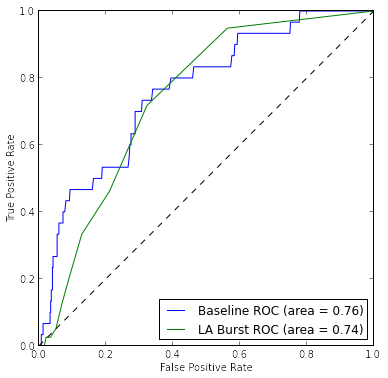
\includegraphics[width=2.1in]{./figures/roc_2013_WorldSeries.png}
\caption{2013 World Series}
\label{fig:roc2013WorldSeries}
\end{subfigure}
\begin{subfigure}[b]{0.3\textwidth}
\centering
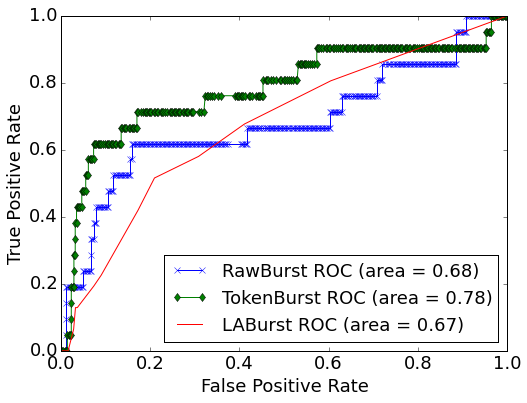
\includegraphics[width=2.1in]{./figures/roc_2014_SuperBowl.png}
\caption{2014 Super Bowl}
\label{fig:roc2014SuperBowl}
\end{subfigure}
\begin{subfigure}[b]{0.3\textwidth}
\centering
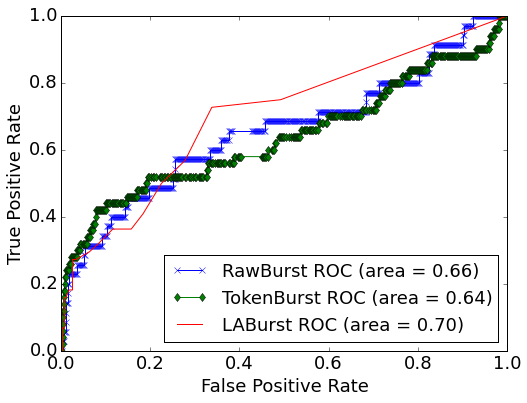
\includegraphics[width=2.1in]{./figures/roc_2014_WorldCup.png}
\caption{2014 World Cup}
\label{fig:roc2014WorldCup}
\end{subfigure}
\caption{Per-Sport ROC Curves}
\label{fig:joinedPerf}
\end{figure*}

\subsection{Composite Results}

To compare comprehensive performance, we look to Figure \ref{fig:rocComprehensive}, which shows ROC curves for all three methods across all three testing events.
From this figure, we see LABurst (AUC=0.71) outperforms RawBurst (AUC=0.65) and performs nearly identically to TokenBurst (AUC=0.72).
Assuming equal cost for false positives and false negatives and optimizing for the largest difference between true positive rate (TPR) and false positive rate (FPR), TokenBurst shows a TPR of 0.5581 and FPR of 0.1408 with a difference of 0.4174 at a threshold value of 13.2.
LABurst, on the other hand, has a TPR of 0.7105 and FPR of 0.3518 with a difference of 0.3587 at a threshold value of 2.
From these values, we see LABurst achieves a higher true positive rate at the cost of a higher false positive rate.
Therefore, it seems the answer to \textbf{RQ1} is that, yes, LABurst can be competitive with existing methods.

\begin{figure}[hbtp]
\begin{center}
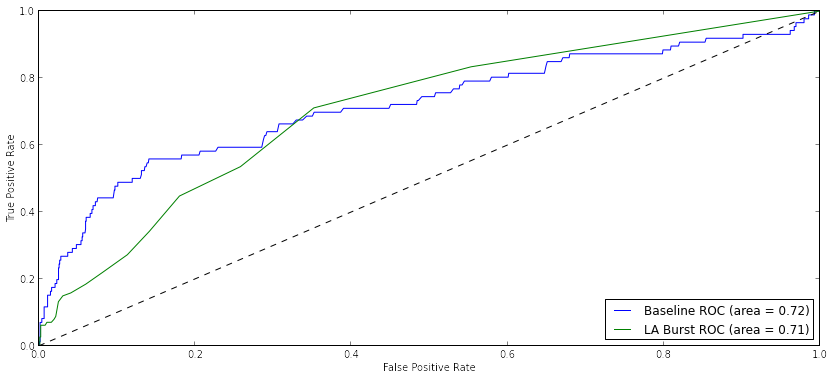
\includegraphics[width=2.75in]{./figures/roc_Comp.png}
\caption{Composite ROC Curves}
\label{fig:rocComprehensive}
\end{center}
\end{figure}

\subsection{Earthquake Detection}

Our second research question (\textbf{RQ2}) seeks to determine whether transferring LABurst's models, as trained on the previously mentioned sporting events, can compete with existing techniques in a different domain.

Figures \ref{fig:2013Japan} and \ref{fig:2014Japan} show the detection curves for both methods for the 2013 and 2014 earthquakes respectively; the red dots indicate the earthquake times as reported by the United States Geological Survey (USGS).
The left vertical axis for each figure reports the frequency of the ``earthquake'' token, and the right axis shows the number of tokens classified as bursty by LABurst.
From the TokenBurst curve, one can see the token ``earthquake'' sees a significant increase in usage when the earthquake occurs, and LABurst experiences a similar increase at the same moment for both events.
It is worth noting that LABurst exhibits bursts prior to the earthquake event, but these peaks \emph{unrelated} to the earthquake event as LABurst does not differentiate between the earthquake and other high-impact events that could be happening on Twitter. 
In addition, the peak occurring about 50 minutes after the earthquake on 25 October 2013 potentially represents an aftershock event\footnote{http://ds.iris.edu/spud/aftershock/9761021}.
Given the minimal lag between the LABurst and TokenBurst's detection, we can answer \textbf{RQ2} in the affirmative. 

\begin{figure*}[btp]
\centering
\begin{subfigure}[b]{0.4\textwidth}
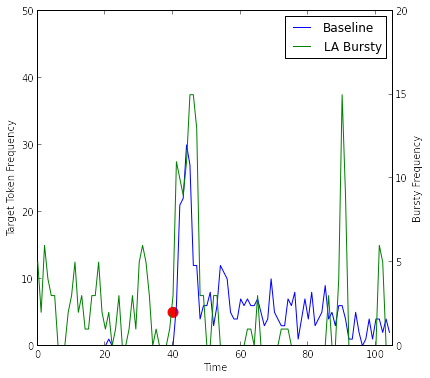
\includegraphics[width=2.25in]{./figures/2013-japan-quake.png}
\caption{Honshu, Japan Earthquake - 25 October 2013}
\label{fig:2013Japan}
\end{subfigure}
\begin{subfigure}[b]{0.4\textwidth}
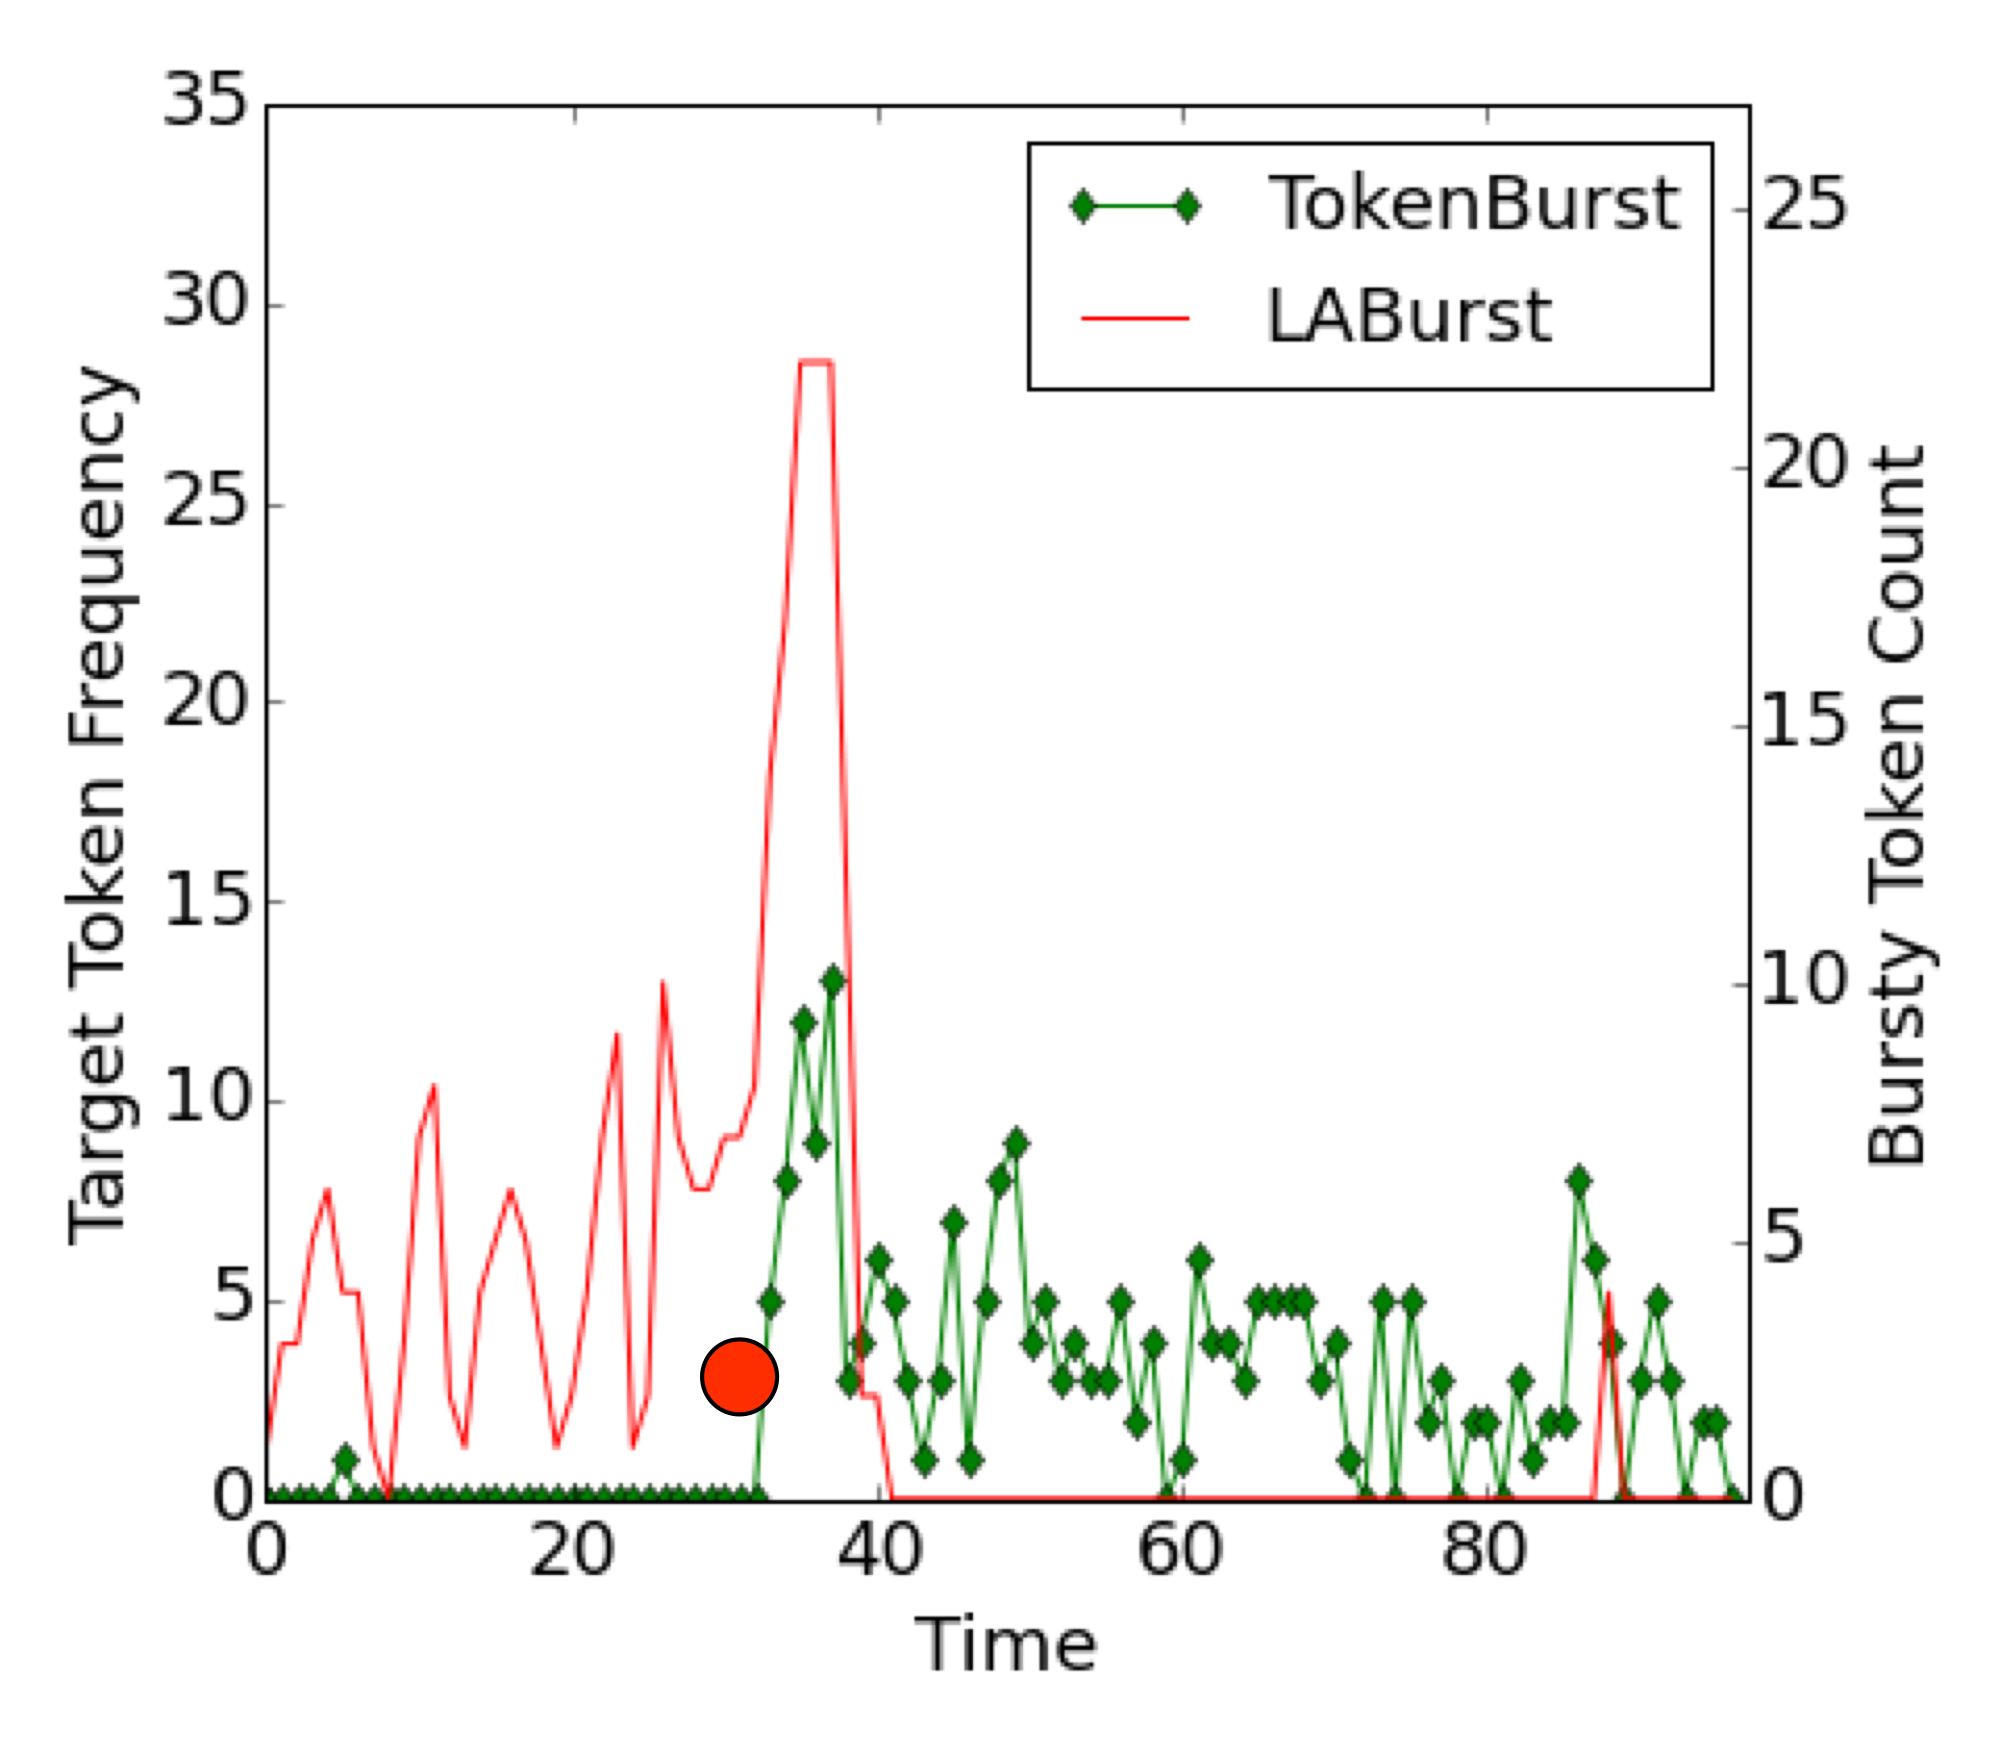
\includegraphics[width=2.25in]{./figures/2014-japan-quake.png}
\caption{Iwaki, Japan Earthquake - 11 July 2014}
\label{fig:2014Japan}
\end{subfigure}
\caption{Japanese Earthquake Detection}
\label{fig:joinedEarthquake}
\end{figure*}

One can now ask what tokens we identified as bursting when the earthquakes occurred.
Many of the tokens are in Japanese, and tokens at the peak of the earthquake events are shown in Table \ref{tab:japanTokens}.
We also extracted several tweets that contain the highest number of these tokens for the given time period, a selection of which include, \begin{CJK}{UTF8}{\myfont}``地震だあああああああああああああああああああああ,'' ``今回はチート使ってないから地震わからなかった,'' and ``地震だー.'' \end{CJK}
Google Translate\footnote{http://translate.google.com} translates these tweets as ``Ah ah ah ah ah ah ah ah ah Aa's earthquake,'' ``I did not know earthquake because not using cheat this time,'' and ``Over's earthquake'' respectively.
%
\begin{table}[htdp]
\caption{Tokens Classified as Busting During Events}
\begin{center}
\begin{tabular}{|p{1.45in} | p{1.45in} |}
\hline
\multicolumn{1}{|c|}{\textbf{Match}} & \multicolumn{1}{|c|}{\textbf{Bursty Tokens}} \\ \hline
Honshu, Japan -- 25 October 2013 & \c{c}dostum, \begin{CJK}{UTF8}{\myfont} 丈, 地, 夫, 怖, 波, 注, 津, 源, 福, 震 \end{CJK} \\ \hline
Iwaki, Japan -- 11 July 2014 & antojo, comida, sammy, \begin{CJK}{UTF8}{\myfont} び, ゆ, ビビ, 地, 怖, 急, 福, 警, 速, 震 \end{CJK} \\ \hline
\end{tabular}
\end{center}
\label{tab:japanTokens}
\end{table}

\section{Analysis}
\label{sect:analysis}

In comparing LABurst with the baseline techniques, it is important to understand the strengths and weaknesses of each baseline: RawBurst requires no prior information but provides little in the way of semantic information regarding detected events, while TokenBurst provides this semantic information at the cost of missing unknown tokens or significant events that do not conform to its prior knowledge.
LABurst combines the benefits of these two approaches in that it not only directly supports undirected event discovery while simultaneously yielding insight into these moments of high interest by tagging relevant bursting tokens.

\subsection{Identifying Event-Related Tokens}

As mentioned, where the baselines require sacrificing flexibility or information, LABurst jointly attacks these problems and yields event-related tokens automatically.
These tokens may include misspellings, colloquialisms, and cross language boundaries, which makes them hard to know before hand.
The 2014 World Cup presents an interesting case for finding these otherwise unexpected tokens because the event has enormous international viewership; as such, many Twitter users of many different languages are likely tweeting about the same event.

To explore the tokens generated during these high-profile events, we look to those tokens identified as bursting during several events in the final two World Cup matches.
Table \ref{tab:burstyTokens} shows a selection of events from these matches and a subset of those tokens classified as bursting during the events (one should note the list is not exhaustive owing to formatting and space constraints).

\begin{table}[htdp]
\caption{Tokens Classified as Busting During Events}
\begin{center}
\begin{tabular}{|p{0.75in}|p{0.7in}| p{1.45in} |}
\hline
\multicolumn{1}{|c|}{\textbf{Match}} & \multicolumn{1}{|c|}{\textbf{Event}} & \multicolumn{1}{|c|}{\textbf{Bursty Tokens}} \\ \hline
Brazil v. Netherlands, 12 July 2014 & Netherlands' Van Persie scores a goal on a penalty at 3', 1-0 & 0-1, 1-0, 1:0, 1x0, card, goaaaaaaal, goal, gol, goool, holandaaaa, k\i{}rm\i{}z\i{}, pen, penal, penalti, p\^{e}nalti, persie, red \\ \hline
Brazil v. Netherlands, 12 July 2014 & Brazil's Oscar get's a yellow card at 68' & dive, juiz, penalty, ref \\ \hline
Germany v. Argentina, 13 July 2014 & Germany's G\"{o}tze scores a goal at 113', 1-0 & goaaaaallllllll, goalllll, godammit, goetze, gollllll, gooooool, gotze, gotzeeee, g\"{o}tze, nooo, yessss, \begin{CJK}{UTF8}{\myfont} ドイツ\end{CJK} \\ \hline
\end{tabular}
\end{center}
\label{tab:burstyTokens}
\end{table}

Several interesting artifacts emerge from this table, first of which is that one can get an immediate sense of the detected event from tokens our algorithm presents. 
For instance, the prevalence of the token ``goal'' and its variations clearly indicate a team scored in the first and third events in Table \ref{tab:burstyTokens}; similarly, bursting tokens associated with the middle event regarding Oscar's yellow card reflect his penalty for diving.
Beyond the pseudo event description put forth by the identified tokens, this reference to diving and to specific player and teams names in the first and third events are also of significant interest.
In the first event, one can infer that the Netherlands scored since ``holandaaaa'' is flagged along with ``persie'' from the Netherlands' player Van Persie, and likewise for Germany's G\"{o}tze in the third event (and the accompanying variations of his name).
These terms would be difficult to capture beforehand as would be required in the baseline and would likely not be related to every event or every type of sporting event.

Finally, the last artifact of note is that the set of bursty tokens displayed includes tokens from several different languages: English for ``goal'' and ``penalty,'' Spanish for ``gol'' and ``penal,'' Brazilian Portuguese for ``juiz'' (meaning ``referee''), as well as the Arabic for ``goal'' and Japanese for ``Germany.''
Since these words are semantically similar but syntactically dissimilar, typical normalization schemes could not capture these connections.
Instead, capturing these words in the baseline would require a pre-specific keyword list in all possible languages or the inclusion of an expensive machine translation system that was also capable of normalizing within different languages (to collapse ``goool'' down to ``gol'' for example).

\subsection{Discovering Unanticipated Moments}
\label{sect:eventDiscovery}

Our experimental results show LABurst is competitive with the domain-specific TokenBurst, but TokenBurst's specificity makes it unable to detect unanticipated moments, and we can see instances of such omissions in the last game of World Cup.
Figure \ref{fig:worldCupFreqs} shows target token frequencies for TokenBurst in green and bursty tokens for our method in red.
From this graph, we can see the first, obvious incidence in Peak \#1 where LABurst exhibits a peak  missed by TokenBurst in the first few points of data.
The primary tokens appearing in this peak are ``puyol,'' ``gisele,'' and ``bundchen,'' which correspond to former Spanish player Carles Puyol and model Gisele Bundchen, who presented the World Cup trophy prior to the match.
At peak \#2, slightly more than eighty minutes into the data (which is sixty minutes into the match), LABurst sees another peak that is otherwise relatively minor in the TokenBurst curve.
Upon further exploration, tokens present in this peak refer to Argentina's substituting in Ag\"{u}ero for Lavezzi at the beginning of the match's second half.

\begin{figure}[hbtp]
\begin{center}
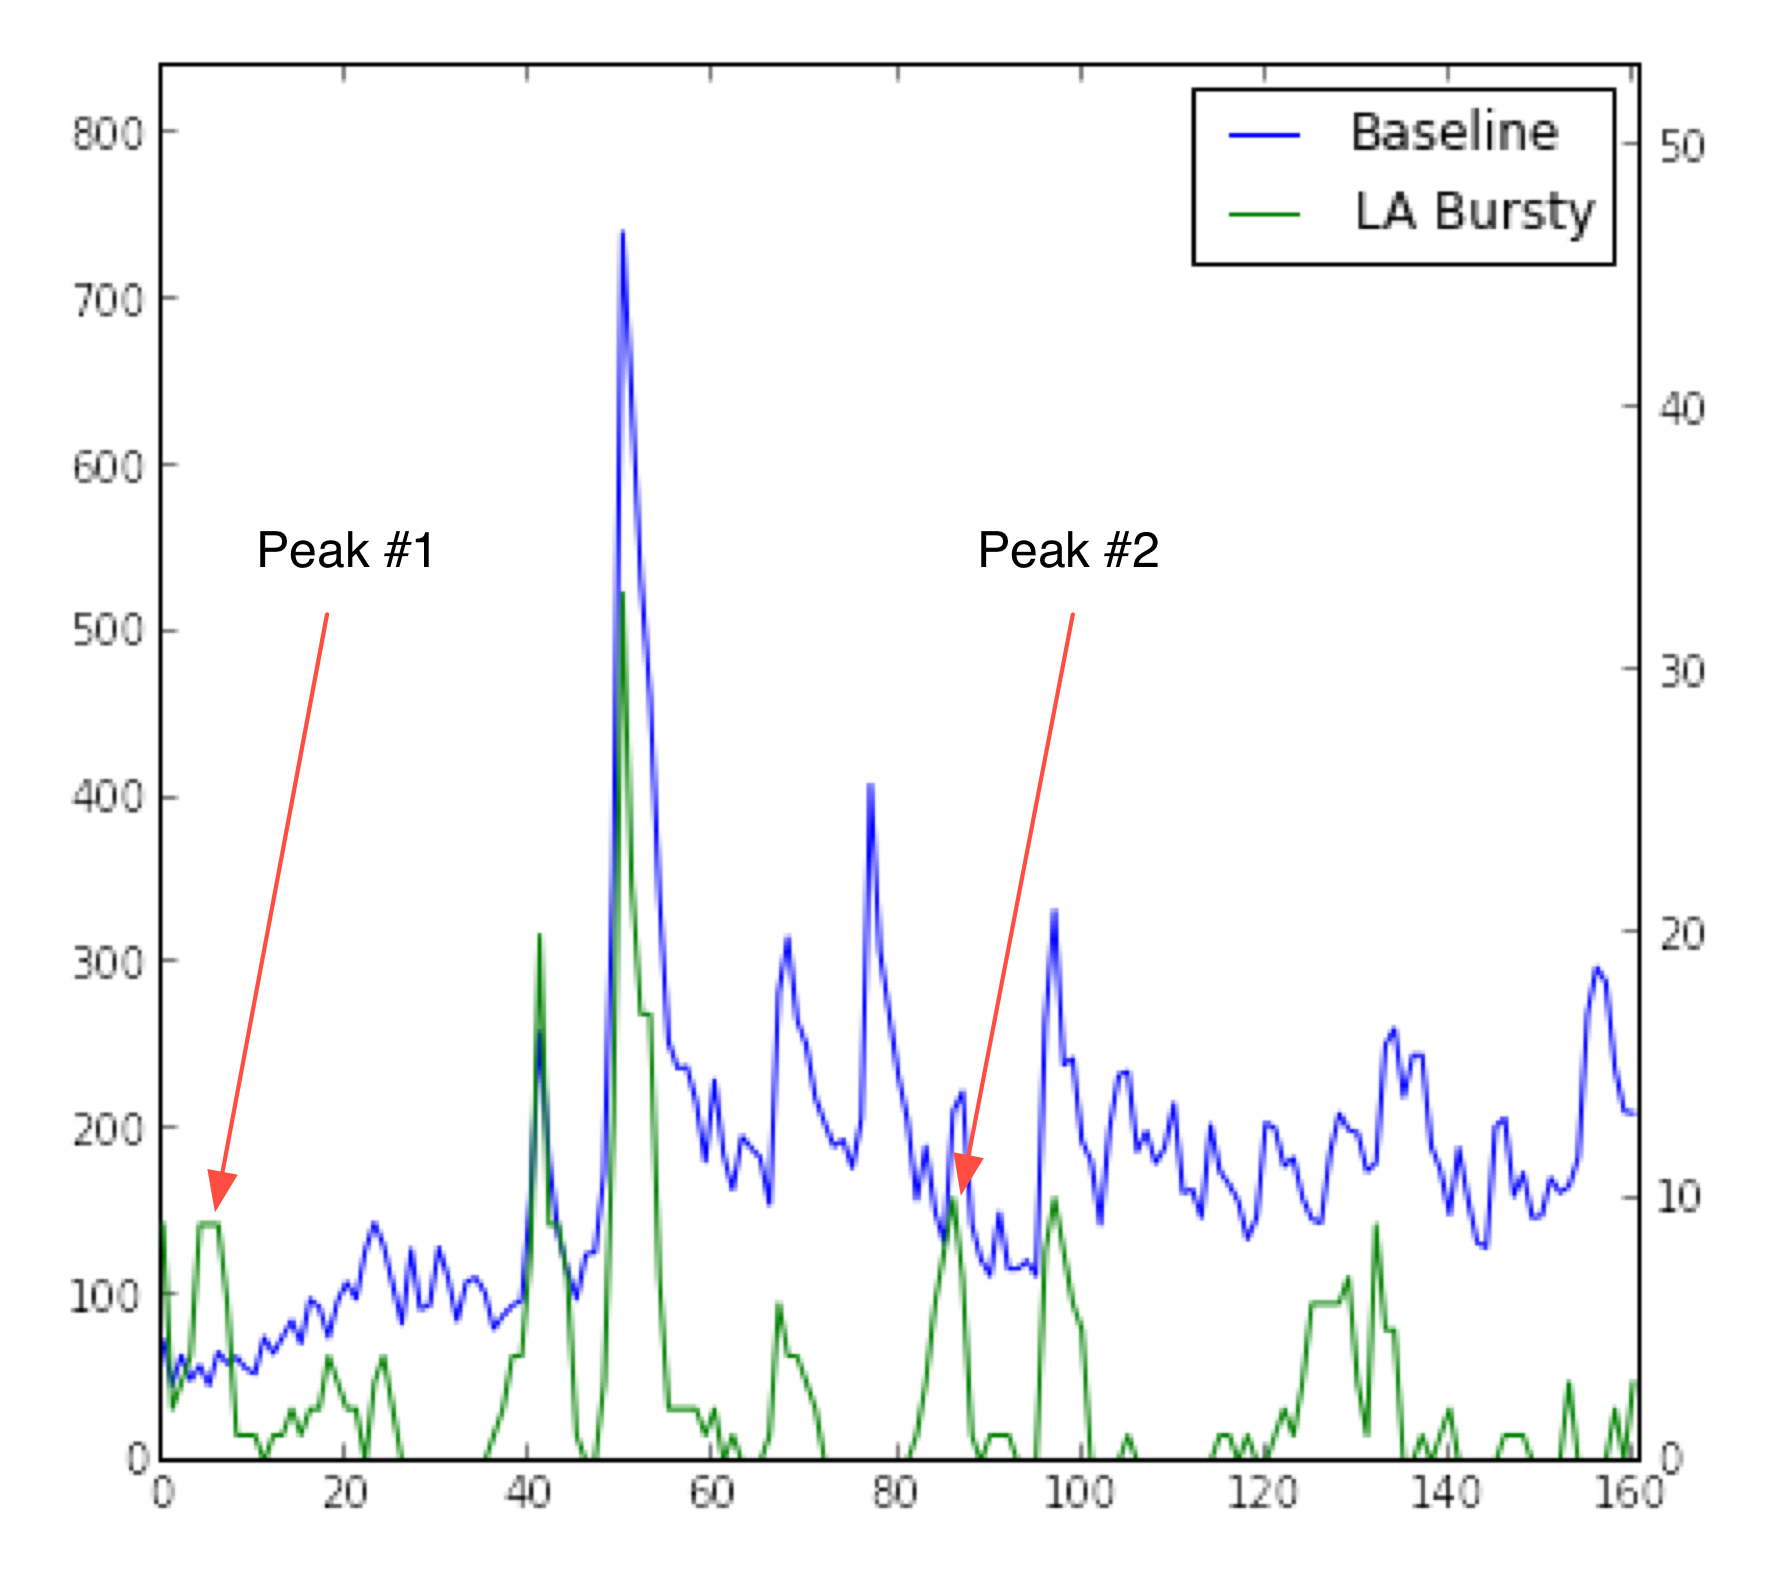
\includegraphics[width=2.75in]{./figures/wc0713freq-labeled.png}
\caption{Baseline and LA Bursty Frequencies}
\label{fig:worldCupFreqs}
\end{center}
\end{figure}

Since LABurst is both language agnostic and domain independent, it likely detects additional high impact events but not part of the game start/end, score, and penalty events present in our ground truth.
For instance, during the Super Bowl, spectators tweet about more moments than just sports plays; they tweet about the half-time show, particularly good or bad commercials, and massive power outages.
Since our ground truth disregards such moments, its higher false-positive rate is perhaps unsurprising.

\section{Conclusions}
\label{sect:conlusions}

To revisit our motivations, the goal for this experiment was to demonstrate the potential of a language-agnostic, machine learning-based approach to discovering highly compelling or interesting moments through analyzing temporal characteristics from unfiltered Twitter data streams.
Our results show that by leveraging temporal characteristics to identify bursty tokens and using the volume of these bursty tokens, we can detect significant events across a collection of disparate sporting competitions and other domains with a level of performance nearly equivalent to an existing, domain-specific baseline.

Similar performance to a baseline is only part of the story, however, as our approach offers notable flexibility in identifying bursting tokens without normalization and across language boundaries.
With this versatility also comes support for event description since we no longer rely on predetermined keywords; that is, we can get a sense of the occurring event by inspecting the bursty tokens.
Finally, these advantages culminate in powerful tool for event \emph{discovery} in that it can unanticipated instances of high interest that we did not expect, regardless of the source language, which makes this technique particularly useful for journalists and newswire sources who have a need to know about events on the ground, as they happen but cannot know a priori what the event may be about in all cases.
In short, this LABurst moment discovery algorithm is able to compete with existing techniques, performs well beyond its training domain, \emph{and} automatically yields tokens describing discovered events.

%\end{document}  % This is where a 'short' article might terminate

%ACKNOWLEDGMENTS are optional
\section{Acknowledgments}
This work made use of the Open Science Data Cloud (OSDC), which is an Open Cloud Consortium (OCC)-sponsored project. 
The OSDC is supported in part by grants from Gordon and Betty Moore Foundation and the National Science Foundation and major contributions from OCC members like the University of Chicago. 

%
% The following two commands are all you need in the
% initial runs of your .tex file to
% produce the bibliography for the citations in your paper.
\bibliographystyle{aaai}
\bibliography{sources}  % sigproc.bib is the name of the Bibliography in this case


\end{document}
